% =============================================================
% Bilgisayar Mimarisi - Kapak Sayfası
% Konsept: Devre Tahtası (PCB) — Fotoğraflı Arka Plan
% =============================================================

% --- Kapak Renkleri ---
\definecolor{pcbzemin}{RGB}{10, 25, 50}
\definecolor{pcbaltin}{RGB}{205, 175, 100}
\definecolor{pcbacik}{RGB}{230, 210, 150}
\definecolor{pcbbeyaz}{RGB}{245, 245, 240}

\begin{titlepage}
\thispagestyle{empty}
\null\vfill
\begin{tikzpicture}[remember picture, overlay]

    % === TAM SAYFA ARKA PLAN GÖRSELİ ===
    % Görsel dikey formatta; genişliği sayfaya sığdır, üst/alttan minimal kırpma
    \begin{scope}
        \clip (current page.south west) rectangle (current page.north east);
        \node[inner sep=0pt] at (current page.center) {%
            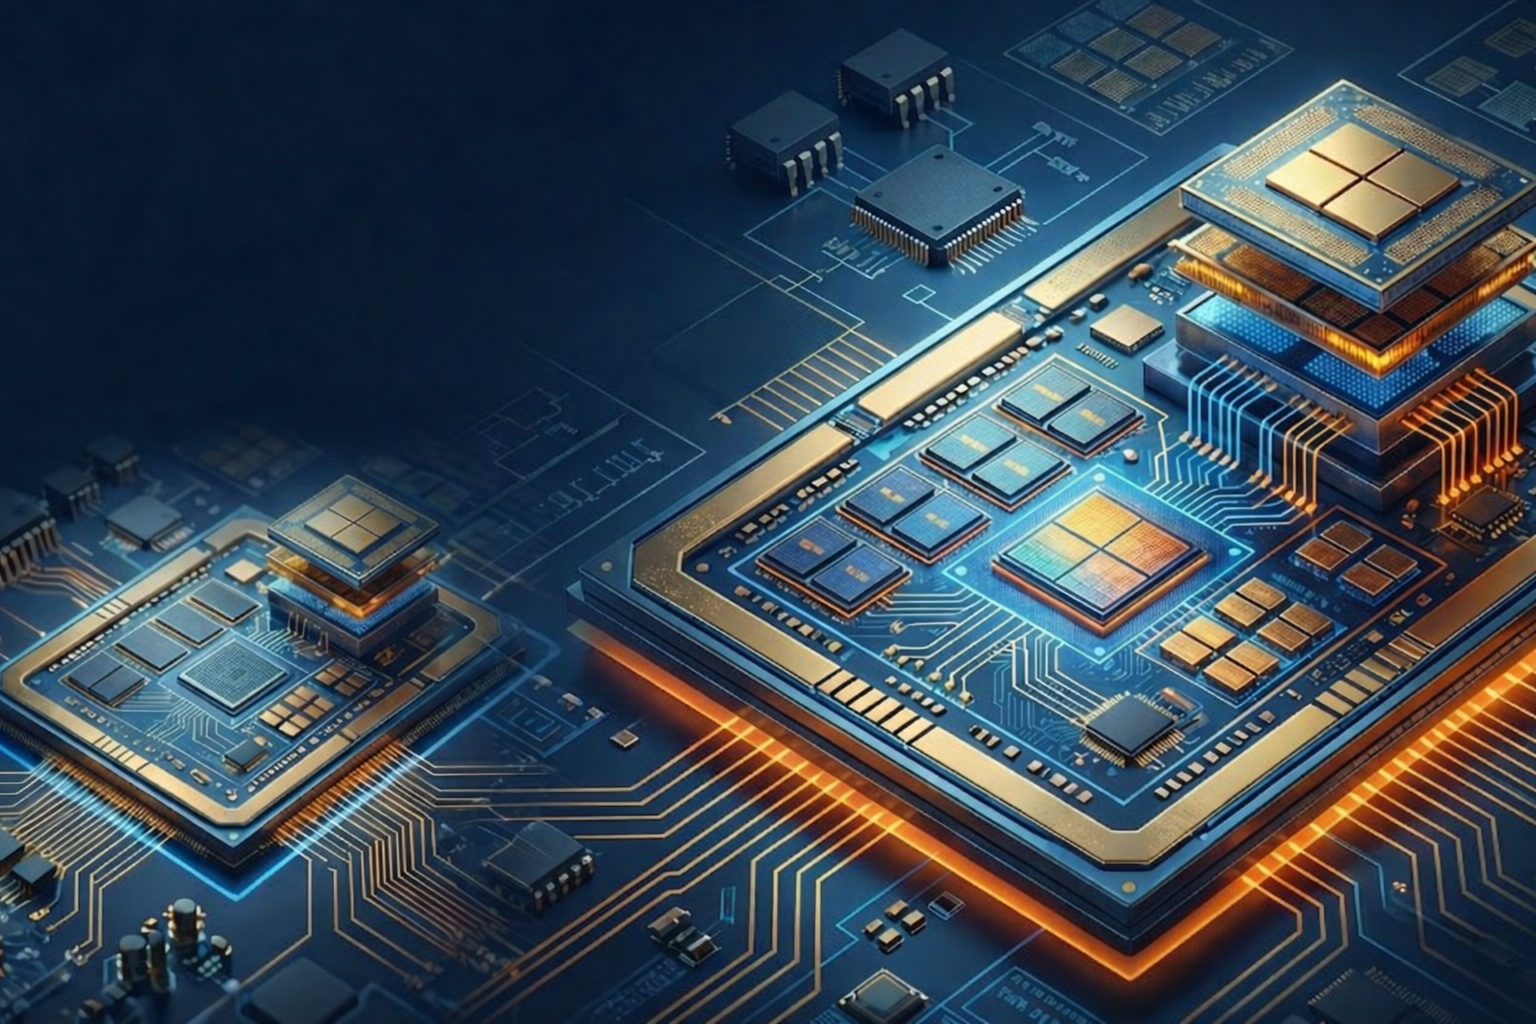
\includegraphics[width=\paperwidth]{gorseller/kapak-arkaplan.png}%
        };
    \end{scope}

    % === ALT BÖLGE: Koyu degrade (metin okunabilirliği için) ===
    % Alt %45: tamamen koyu
    \fill[pcbzemin, opacity=0.85]
        (current page.south west) rectangle ([yshift=13.5cm]current page.south east);
    % Kademeli geçiş bantları (yumuşak degrade etkisi)
    \fill[pcbzemin, opacity=0.7]
        ([yshift=13.5cm]current page.south west) rectangle ([yshift=14.5cm]current page.south east);
    \fill[pcbzemin, opacity=0.5]
        ([yshift=14.5cm]current page.south west) rectangle ([yshift=15.5cm]current page.south east);
    \fill[pcbzemin, opacity=0.3]
        ([yshift=15.5cm]current page.south west) rectangle ([yshift=16.5cm]current page.south east);
    \fill[pcbzemin, opacity=0.15]
        ([yshift=16.5cm]current page.south west) rectangle ([yshift=17.5cm]current page.south east);

    % === ÜST ŞERİT (ince altın çizgi) ===
    \fill[pcbaltin] (current page.north west) rectangle ([yshift=-1.2mm]current page.north east);

    % === ALT ŞERİT (ince altın çizgi) ===
    \fill[pcbaltin] ([yshift=1.2mm]current page.south west) rectangle (current page.south east);

    % === ANA BAŞLIK ===
    \node[font=\fontsize{42}{50}\selectfont\bfseries, text=pcbbeyaz]
        at ([yshift=9.5cm]current page.south) {Bilgisayar};
    \node[font=\fontsize{42}{50}\selectfont\bfseries, text=pcbbeyaz]
        at ([yshift=7.5cm]current page.south) {Mimarisi};

    % === ALTIN AYIRICI ÇİZGİ ===
    \draw[pcbaltin, line width=1.2pt]
        ([yshift=6.5cm, xshift=-3cm]current page.south) -- ++(6cm,0);

    % === ALT BAŞLIK ===
    \node[font=\Large\itshape, text=pcbacik]
        at ([yshift=5.5cm]current page.south) {RISC-V Tabanlı Yaklaşım};

    % === YAZAR ADI ===
    \node[font=\large\bfseries, text=pcbbeyaz]
        at ([yshift=3.8cm]current page.south) {Prof.\ Dr.\ Oğuz Ergin};

    % === BASKI BİLGİSİ ===
    \node[font=\normalsize, text=pcbaltin, opacity=0.7]
        at ([yshift=1.8cm]current page.south) {Sürüm 0.2.0\ \ $\cdot$\ \ \the\year};

\end{tikzpicture}
\vfill
\end{titlepage}
